\documentclass[12pt,a4paper]{article}
\usepackage[left=2.50cm, right=1.00cm, top=1.00cm, bottom=2.00cm]{geometry}
\usepackage[utf8]{inputenc}
\usepackage[T2A]{fontenc}
\usepackage[english, russian]{babel}
\usepackage{amsmath, amsfonts, amssymb}
\usepackage{graphicx}
\usepackage[most]{tcolorbox}
\usepackage{mathrsfs}
\usepackage{alltt}

\begin{document}
\selectlanguage{russian}

\setcounter{section}{13}
\section{Рекурсия}

\subsection{Основные понятия}

\textbf{Рекурсия} ---  определение, описание, изображение какого-либо объекта или процесса внутри самого этого объекта или процесса.

В математике рекурсия имеет отношение к методу определения функций и числовых рядов: рекурсивно заданная функция определяет своё значение через обращение к себе самой с другими аргументами. 

Классический пример: рекурсивно-определённый факториал целого неотрицательного числа:
$$
n!= \begin{cases}
	1 & \text{для}\ n=0,\\
	n*(n-1)! & \text{для}\ n>0
	\end{cases}
$$
Поскольку $n$, по определению, целое неотрицательное число, через $n$ рекурсивных обращений вычисление функции гарантированно придёт к частному случаю $0!=1$, на котором рекурсия прекратится. Таким образом, несмотря на рекурсивность определения, вычисление функции для любого аргумента из области определения окажется конечным.

\subsection{Нисходящая рекурсия}

В программировании подпрограмма может вызывать сама себя, и тогда подпрограмма будет являться рекурсивной.

Рассмотрим пример вычисления факториала по описанной ранее формуле при помощи функции:

\begin{alltt}
//Функция расчета факториала
//при помощи рекурсии
//Входные значения:
//  n - значение аргумента,
//      должно быть неотрицательным
//Входные значения:
//  f\_down - значение факториала
1 function f\_down(n: integer):integer;
2 begin
3  if n = 0 then //терминальная ситуация
4    f\_down := 1
5  else
6    f\_down := n * f\_down(n - 1);
7 end;
\end{alltt}

В строке (3) описана так называемая \textbf{терминальная ситуация} --- это условие в рекурсивном алгоритме вычислений при котором значение может быть вычислено без рекурсивного обращения. Для вычисления факториала такой терминальной ситуацией будет вычисление $0!$. 
В строке (6)  в операторе присваивания в левой части стоит имя функции, а в правой --- выражение, содержащее обращение к этой же функции с аргументом $(n-1)$. 

Добавим в текст операторы для промежуточных вычислений и вывода, чтобы посмотреть, как будет вычисляться значение факториала:

\begin{alltt}
1 function f\_down(n: integer):integer;
2 var
3   r: integer;
4 begin
5   WriteLn('f\_down (in) n = ', n);
6   if n = 0 then //терминальная ситуация
7     f\_down := 1
8   else
9     begin
10      //вычисление по формуле n! = n*(n-1)!
11      r := n * f\_down(n - 1);
12      Writeln('Current result is = ', r);
13      f\_down := r;
14    end;
15    WriteLn('f\_down (out) n = ', n);
16 end;
17 var 
18   f, n: integer;
19 begin
20   Write('Factorial calculation, input n = ');
21   ReadLn(n);
22   Writeln('Using downward recursion');
23   f := f\_down(n);
24   WriteLn('Result: ', n, '! is ', f);
25   Writeln;
26   Write('Press Enter to quit...');
27   ReadLn;
28 end.
\end{alltt}

В функции мы сначала в строке (5) печатаем значение аргумета, потом - значение вычисленного результата (12), потом --- значение аргумента при завершении функции. Результат показан на рисунке \ref{pic01}.

\begin{figure}[ht!]
	\centering	
	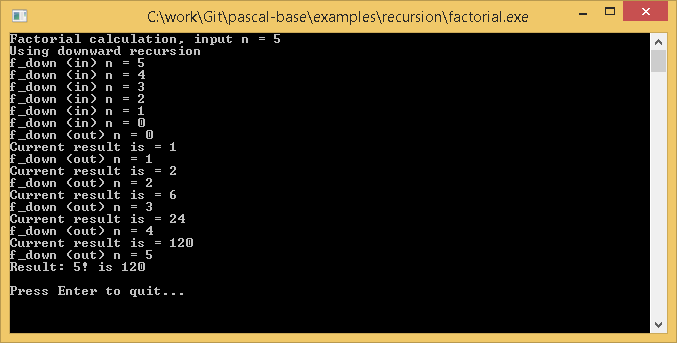
\includegraphics[width=0.9\textwidth]{images/lec14-pic01.png}
	\caption{Результат выполнения программы расчета факториала. Нисходящая рекурсия}
	\label{pic01}
\end{figure}

На рисунке видно, что сначала идут последовательные вызовы функции с уменьшением параметра $n$. Потом вычисление доходит до терминальной ситуации при $n=0$, и затем начинается последовательный возврат значений и завершение вызовов функций. После завершения вызова исходной функции в основную программу мы получаем результат - $5!=120$.

Данный вид рекурсии называется \textbf{нисходящей рекурсией} --- в ней процесс вычислений осуществляется на <<обратном ходе>> вычислительного процесса.

\subsection{Восходящая рекурсия}

Рассмотрим текст программы, в которой реализовна \textbf{восходящая рекурсия} вычисления факториала.

\begin{alltt}
//Процедура расчета факториала при помощи восходящей рекурсии
//Входные значения:
//  n - значение аргумента,
//      должно быть неотрицательным
//Входные значения:
//  res - накапливаемое значение факториала
1 procedure f\_up(n: integer; var res: integer);
2 begin
3   WriteLn('f\_up (in) n = ', n);
4   if n = 0 then //терминальная ситуация
5     exit
6   else
7     begin
8       Writeln('Current (in) result is = ', res);
9       res := res * n;
10      f\_up(n-1, res);
11      Writeln('Current (out) result is = ', res);
12    end;
13    WriteLn('f\_up (out) n = ', n);
14 end; 
15 var
16   f, n: integer;
17 begin
18   Write('Factorial calculation, input n = ');
19   ReadLn(n);
20   Write('Using upward recursion');
21   //начальное значение f должно быть инициализированно
22   f := 1;
23   f\_up(n, f);
24   WriteLn('Result: ', n, '! is ', f);
25   Writeln;
26   Write('Press Enter to quit...');
27   ReadLn;
28 end.
\end{alltt}

В данной программе имеются следующие отличия:
\begin{itemize} 
	\item вместо функции используется процедура, так как для передачи рассчитанного значения будет использоваться параметр подпрограммы $res$;
	\item непосредственно вычисление факториала будет происходить в строке (9), где текущее расситанное значение будет умножено на параметр $n$;
	\item далее в строке (10) происходит рекурсивный вызов, для расчета факториала со значением параметра $n-1$;
	\item так как для расчета используется параметр-переменная, то необходима ее предварительная инициализация (в строке (22));
\end{itemize}	

\begin{figure}[h!]
	\centering	
	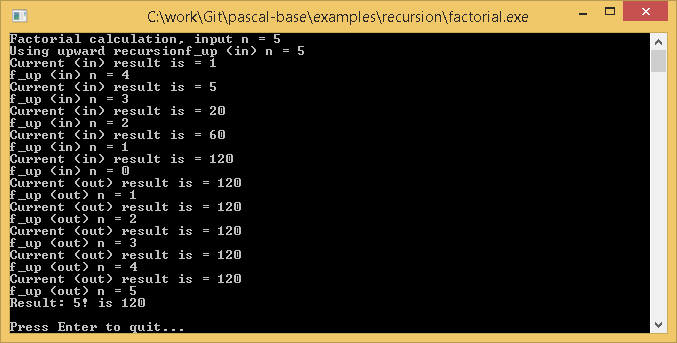
\includegraphics[width=0.9\textwidth]{images/lec14-pic02.png}
	\caption{Результат выполнения программы расчета факториала. Восходящая рекурсия}
	\label{pic02}	
\end{figure}

На рисунке \ref{pic02} видно, что вычисление происходит на прямом ходе рекурсии, факториал вычисляется на шестом реккрсивном вызове, после чего все процедуры последовательно завершаются.

Правильно написанная рекурсивная функция должна гарантировать, что через конечное число рекурсивных вызовов будет достигнуто выполнение условия прекращения рекурсии, в результате чего цепочка последовательных рекурсивных вызовов прервётся и выполнится возврат.

Пример с факториалом --- во многом искусственный, так как существует простой итерационный способ вычисления факториала как произведения последовательный натуральных чисел: 
$$n!=\prod_{i=1}^{n}i$$.

И алгоритм вычисления очень прост:

\begin{alltt}
	1 var
	2   i, n, f: integer;
	3 begin
	4   Write('Factorial calculation, input n = ');
	5   ReadLn(n);
	6   Write('Using iterations:');
	7   f := 1;
	8   for i:=2 to n do
	9     f := f * i;
	10   Write('Press Enter to quit...');
	11   ReadLn;
	12 end.
\end{alltt}

Несмотря на то, что описание алгоритма в рекурсивном виде во многих задачах (которые будут рассмотрены далее) выглядит кратко и элегантно, на практике реализацию алгоритма делают при помощи итерационных процессов. 

Реализация рекурсивных вызовов функций опирается на механизм стека вызовов --- адрес возврата и локальные переменные функции записываются в стек, благодаря чему каждый следующий рекурсивный вызов этой функции пользуется своим набором локальных переменных и за счёт этого работает корректно. Объем стека ограничен, и если глубина рекурсии будет большой, то в стеке может закончится место, что приведет к ошибке \texttt{stack overflow}.

Теоретически, любую рекурсивную функцию можно заменить циклом и стеком. 

\subsection{Параллельная рекурсия}

Рекурсия называется \textbf{параллельной}, если в рекурсивной ветви алгоритма происходит несколько рекурсивных вызовов.

Рассмотрим пример вычисления $n$-го числа Фибоначчи. Числа Фибоначчи задаются при помощи следующей рекурсивной формулы:

$$
\begin{cases}
f_0 = 1,\\
f_1 = 1,\\
f_n = f_{n-1}+f_{n-2}\ \text{для}\ n>1
\end{cases}
$$

Напишем рекурсивный алгоритм вычисления $n$-го числа Фибоначчи:

\begin{alltt}
	//Рекурсивная функция вычисления n-го
	//числа Фибоначчи
	//Входные параметры:
	//  n - номер числа (n>=0)
	//Выходное значение:
	//  f\_req - число Фибоначчи
1	function f\_req(n: integer): integer;
2	begin
3 	  if (n = 0) or (n = 1) then
4	    f\_req := 1
5	  else
6	    f\_req := f\_req(n-1) + f\_req(n-2)
7	end;
\end{alltt}

В строке (6) в правой части оператора присваивания находятся два вызова функции : \texttt{f\_req(n-1)} и \texttt{f\_req(n-2)}. Несмотря на название --- <<параллельная рекурсия>>, эти вызовы не будут выполняться одновременно. Доработаем наш алгоритм, добавив вывод информации о вызове фукнций и расчет общего количества вызовов.

\begin{alltt}
	//Рекурсивная функция вычисления n-го
	//числа Фибоначчи
	//Входные параметры:
	//  n - номер числа (n>=0)
	//Выходное значение:
	//  f\_req - число Фибоначчи
	//  n\_count - глобальная переменная,
	//            счетчик вызовов функции	
1	var
2	  n\_count: integer; //счетчик итераций для рекурсивной функции	
3	function f\_req(n: integer): integer;	
4	begin
5	  inc(n_count);
6	  WriteLn('Call f (', n, ')');	
7	  if (n = 0) or (n = 1) then
8	    f\_req := 1
9	  else
10	    f\_req := f\_req(n-1) + f\_req(n-2)
11	end;
12	var
13    n, fn: integer;
14	begin
15	  Write('Input n = ');
16	  ReadLn(n);
17	  n\_count := 0;
18	  fn := f\_req(n);
19	  WriteLn(n, '-th Fib number is ', fn);
20	  WriteLn('We need ', n\_count, ' function call in requsive case!');
21	end.	
\end{alltt}

Результат запуска рекурсивной программы для расчета числа Фибоначчи представлен на рисунке \ref{pic03}. Для расчета $f_7$ потребовлся $41$ вызов функции \texttt{f\_req(n)}. 

Для вычисления \textit{седьмого} числа Фибоначчи потребовался \textit{двадцать один} вызов функции. 

Если построить график зависимости количества вызовов функции в зависимости от порядкового номера числа, то мы получим график, представленный на рисунке \ref{pic04}. На графике видно, что зависимость количества вызовов от числа является экспоненциальной. 

\begin{figure}[h!]
	\centering	
	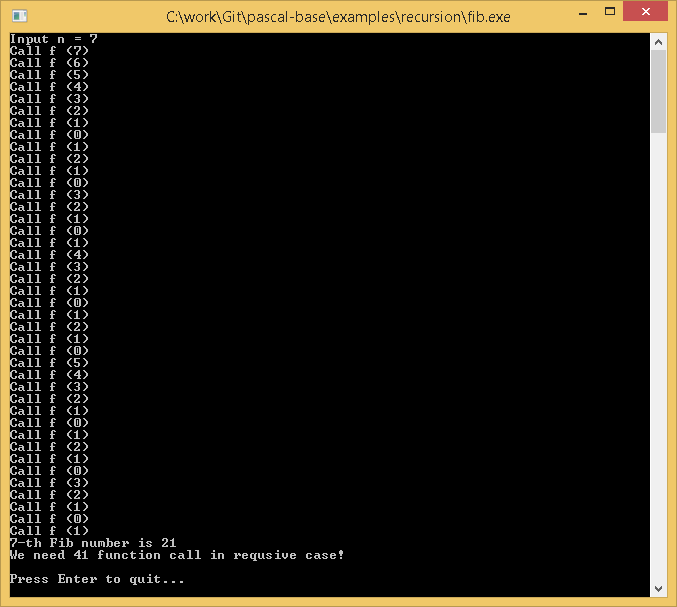
\includegraphics[width=0.9\textwidth]{images/lec14-pic03.png}
	\caption{Результат выполнения программы расчета числа Фибоначчи. Параллельная рекурсия}
	\label{pic03}	
\end{figure}

\begin{figure}[h!]
	\centering	
	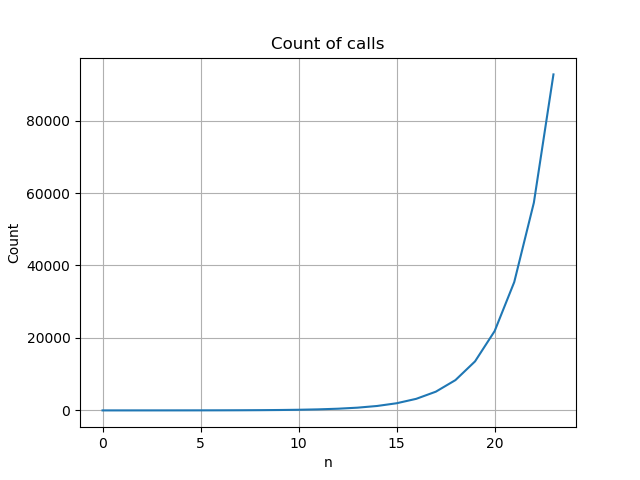
\includegraphics[width=0.9\textwidth]{images/lec14-pic04.png}
	\caption{Зависимость количества вызовов функции f\_req от номера числа Фибоначчи}
	\label{pic04}	
\end{figure}

Для задачи вычисления числа Фибоначчи также существует простой итерационный алгоритм, который потребует всего две вспомогательные переменные для хранения значений чисел Фибоначчи, вычисленных на двух предыдущих шагах:

\begin{alltt}
//Итерационная функция вычисления числа Фибоначчи
1  function f\_iter(n: integer): integer;
2  var
3    i: integer;
4    a, b, c: integer;
5  begin
6    a := 1; b := 1;
7    for i := 2 to n do
8    begin
9      c := b + a;
10     a := b;
11     b := c;
12   end;
13   f\_iter := b;
14 end; 	
\end{alltt}

Рассмотрим следующую задачу, в которой покажем, как хранение промежуточных результатов вычислений поможет сократить число рекурсивных вызовов и увеличить скорость расчетов. 

\begin{tcolorbox}
	\textbf{Задача}: необходимо определить, сколько существует различных способов разменять сумму в $N$ рублей монетами достоинством 1, 5 и 10 рублей. Примечание: варианты, которые отличаются порядком монет (например, 1-10-5-1 и 5-10-1-1 считаются различными).
\end{tcolorbox}

Данная задача имеет простое решение: для того, чтобы посчитать количество вариантов для размена суммы в N рублей, мы должны сложить варианты размена сумм (N-1), (N-5) и (N-10).

\begin{alltt}
1	function variants(sum: integer):integer;
2	begin
3	  if sum < 0 then
4	    variants := 0
5	else
6	    if sum = 0 then
7	      variants := 1
8	    else
9	      variants := variants(sum-1) + variants(sum-5) + variants(sum-10);
10	end;
\end{alltt}

В строке (9) в правой части оператора присваивания присутствует \textit{три} рекурсивых вызова, и количество рекурсивных вызовов будет больше, чем при вычислении числа Фибоначчи. Рассмотрим пример реализации алгоритма вычислений, который будет использовать глобальный массив для хранения результатов вычислений, что приведет к соращению числа рекурсвиных вызовов. 

\begin{alltt}
1 var
2   calls: integer;
3 function variants(sum: integer):integer;
4   const
5     NO\_DATA = -1;
6   var
7     counts: array of integer;
8     i: integer;
9   function calc\_variants(sum: integer):integer;
10  begin
11    inc(calls);
12    if sum < 0 then
13      calc\_variants := 0
14    else
15      if sum = 0 then
16        calc\_variants := 1
17      else
18        begin
19          if counts[sum] = NO\_DATA then
20            counts[sum] := calc\_variants(sum-1) 
21              + calc\_variants(sum-5) 
22              + calc\_variants(sum-10);
23          calc\_variants := counts[sum];
24        end;
25  end;
26  begin
27    SetLength(counts, sum+1);
28    for i := 0 to sum do
29      counts[i] := NO\_DATA;
30    variants := calc\_variants(sum);
21  end;   
\end{alltt}

Рассмотрим данную реализацию:
\begin{itemize}
	\item в строке (2) описана глобальная переменная для подстчета числа обращений к функции;
	\item функция variants содержит блок описания констант, переменных и рекурсвиную функцию calc\_variants;
	\item в строке (5) описана констанат NO\_DATA для описания факта, что для заданной суммы количество вариантов еще не расчитывалось;
	\item в строке (7) описан глобальный для функции  calc\_variants массив \texttt{counts}, который будет будет хранить результаты промежуточных вычислений;
	\item функция calc\_variants выполняет вычисление по следующему алгоритму:
	\begin{enumerate}
		\item в (11) увеличивается зачение счетчика вызовов;
		\item в (12) проверяется условие $sum<0$ (аналогичное рекурсвному вызову);
		\item в (15) проверяется условие $sum=0$ (аналогичное рекурсвному вызову);	
		\item в (19) осуществляется проверка $counts[sum] = NO\_DATA$ --- что для значения для $sum$ не было рассчитано значение количества вариантов;
		\item если значение не было рассчитано, то осуществляется расчет с обращением к рекурсивным вызовам (20-22);
		\item в(20) в элемент массива будет записан результат расчета, который будет использоваться, если будет необходимость в получении ранее рассчитанного значения;
		\item в строке (23) возвращается значение (либо ранее рассчитанное, либо вычисленное);
		\item в (27) задается размер глобального массива \texttt{counts}, который используется для хранения промежуточных вычислений;
		\item в (28, 29) инициализируется массив значений (в каждый элемент записывается признак NO\_DATA); 
		\item в (30) в качестве значения функции возвращается результат расчета --- через обращение к локальной функции  calc\_variants.
	\end{enumerate}
\end{itemize}

\begin{figure}[h!]
	\centering	
	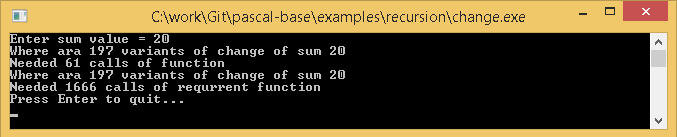
\includegraphics[width=0.9\textwidth]{images/lec14-pic05.png}
	\caption{Результат расчета количества вариантов размена при помощи рекурсивной функции и рекурсвиной функции с использованием вспомогательного глобального массива}
	\label{pic05}	
\end{figure}

Использование дополнительной памяти позволило сократить количество рекурсивных вызовов за счет выделения дополнительной памяти. Как правило, во всех задачах приходится искать компромисс между использованием памяти и скоростью работы алгоритма.

\begin{alltt}
	1	function variants(sum: integer):integer;
	2	begin
	3	  if sum < 0 then
	4	    variants := 0
	5	else
	6	    if sum = 0 then
	7	      variants := 1
	8	    else
	9	      variants := variants(sum-1) + variants(sum-5) + variants(sum-10);
	10	end;
\end{alltt}

В строке (9) в правой части оператора присваивания присутствует \textit{три} рекурсивых вызова, и количество рекурсивных вызовов будет больше, чем при вычислении числа Фибоначчи. Рассмотрим пример реализации алгоритма вычислений, который будет использовать глобальный массив для хранения результатов вычислений, что приведет к соращению числа рекурсвиных вызовов. 

\subsection{Бинарный поиск}

Рассмотрим алгоритм бинарного поиска в упорядоченном массиве значений.

\begin{tcolorbox}
	Пусть задан упорядоченный (по возрастанию) набор значений $a_1, a_2, \dots, a_n$. Требуется определить, имеется ли в данном наборе значений значение $value$.
\end{tcolorbox}

Алгоритм бинарного поиска можно описать следующим образом:
\begin{enumerate}
	\item задаем начальные границы поиска \texttt{left=1, right=n}; 
	\item вычисляем середину последовательности \texttt{middle};  
	\item если элемент с индексом \texttt{middle} равен искомому, то завершаем алгоритм, возвращаем принзнак, что элемент найден;
	\item если элемент 	с индексом \texttt{middle} больше искомого, то осуществляем бинарный поиск в границах (left, middle-1)
	\item если элемент 	с индексом \texttt{middle} меньше искомого, то осуществляем бинарный поиск в границах (middle+1, right)	
	\item поиск завершается неудачей, если левая граница оказывается больше правой.		
\end{enumerate}

Текст программы бинарного поиска представлен ниже.

Функция рекурсивного поиска описана в строках (3-21). В строке (7) выводится отладочная информация. 

В строке (12) осуществляется расчет зачения середины. Обратите внимание, что использовалась конструкция \texttt{middle := left + (right - left) div 2}, так как вычисление значения выражения \texttt{(right + left) div 2} может привести к переполнению значений - сумма \texttt{right + left} может выйти за пределы максимального значения типа.

В строках (17) и (19) осуществляются рекурсивные вызовы для поиска в левой и правой частях массива соответственно.

В строках (22-24) описана функция, которая вызывает рекурсивную функцию бинарного поиска с начальными параметрами.

В разделе операторов осуществляется проверка работы функции бинарного поиска - осуществляется поиск значений, как присутствующих в заданном наборе, так и отсутствующих в нем.

\begin{alltt}
1	type
2	  TArray = array of integer;	
3	function search\_req(const arr: TArray; left, right, key: integer): integer;
4	var
5	  middle: integer;
6	begin
7	  Writeln('find ', key, ' left = ', left, ' right = ', right);	
8	  if right < left then
9	    search\_req := -1
10	  else
11	    begin
12	      middle := left + (right - left) div 2; //(right + left) div 2;	
13	      if arr[middle] = key then
14	        search\_req := middle
15	      else
16	        if arr[middle] > key then
17	          search\_req := search\_req(arr, left, middle-1, key)
18	        else
19	          search\_req := search\_req(arr, middle+1, right, key);
20	    end;
21    end;	
22	function search(const arr: TArray; key: integer): integer;
22	begin
23	  Result := search\_req(arr, 0, length(arr), key);
24	end;	
25	procedure print\_array(const arr: TArray);
26	var
27	  i: integer;
28	begin
29	  for i := 0 to High(arr) do
30	    Write(arr[i], ' ');
31	  WriteLn;
32	end;
33	procedure test\_search(const arr: TArray; key: integer);
34	var
35 	  index: integer;
36	begin
37	  WriteLn('Trying to find ', key, ' in array: ');	
38	  index := search(arr, key);	
39	  WriteLn('Result index is ', index);
40	  WriteLn;
41	end;
42	var	a: TArray;	
43	begin
44	  a := TArray.Create(0, 1, 2, 2, 2, 4, 4, 5, 5, 5);	
45	  Write('Array is ');
46	  print\_array(a);	
49	  test\_search(a, 1);
55	  Write('Press Enter to quit...');
56	  ReadLn;
57	end.
\end{alltt}

Результат выполнения программы для поиска значения 1 показан на рисунке \ref{pic06}.

\begin{figure}[h!]
	\centering	
	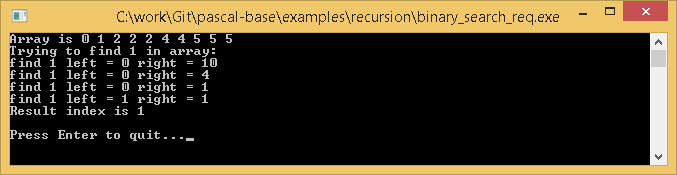
\includegraphics[width=0.9\textwidth]{images/lec14-pic06.png}
	\caption{Результат выполнения бинарного поиска}
	\label{pic06}	
\end{figure}

Несмотря на то, что данная реализация алгоритма также рекусивная, даже такая реализация может быть использована в программах, так как с каждым последующим рекурсивным вызовом количество элементом уменьшается в два раза. Таким образом, для массива из $N$ элементов потребуется максимум $log_2(N)$ рекурсивных вызовов. Например, для массива из 1024 элементов потребуется макисмум 5 вызовов функции, чтобы определить наличие или отсутствие искомого элемента.

Бинарный поиск также может быть реализован в виде итерационного алгоритма. В следующем примере приведены две функции, которые вычисляют границы (левую и правую), внутри которых лежит искомое(искомые) значения.

Если в наборе значений искомое значение (например, 2) встречается несколько раз (например, в наборе: 0, 1, 2, 2, 2, 3, 7, 12), то функция \texttt{left\_bound} вернет значение индекса = 1, в функция \texttt{right\_bound} --- значение 5.

\begin{alltt}
1	function left\_bound(arr: array of integer; key: integer): integer;
2	var
3	  left, right, middle: integer;
4	begin
5	  left := -1;
6	  right := length(arr);
7	  while right - left > 1 do
8	  begin
9	    middle := left + (right - left) div 2;
10	    if arr[middle] < key then
11	      left := middle
12	    else
13	      right := middle;
14	  end;
15	  Result := left;
16	end;

17	function right\_bound(arr: array of integer; key: integer): integer;
18	var
19	  left, right, middle: integer;
20	begin
21	  left := -1;
22	  right := length(arr);
23	  while right - left > 1 do
24	  begin
25	    middle := left + (right - left) div 2; 
26	    if arr[middle] <= key then
27	      left := middle
28	    else
29	      right := middle;
30	  end;
31	  Result := right;
32	end;
\end{alltt}

На основе рекурсии построен алгоритм \textit{быстрой сортировки}, но для его рассмотрения необходима целая лекция. 

\section*{Контрольные вопросы}

\begin{enumerate}
	\item В чем отличие восходящей рекурсии от нисходящей?
	\item Может ли в рекурсивной функции отсутствовать терминальная ситуация?
	\item В чем недостаток рекурсивных алгоритмов по сравнению с итерационными? В чем преимущество?
	\item Определите характер зависимости ($y=f(n)$) между количеством рекурсивных вызовов и входным параметром N для алгоримта вычисления числа N-ого числа Фибоначчи. Характер зависимости может быть: линейным, полиномиальным, экспоненциальным и т.д.
	\item Сравните время выполнения алгоритмов бинарного поиска для итерационной и рекурсивной реализации.
	\item В реализации алгоритма бинарного поиска с функциями \texttt{left\_bound} и \texttt{right\_bound}, определите: 
	\begin{itemize}
	\item количество искомых элементов в массиве;
	\item отсутсвие искомого элемента в массиве;	
	\end{itemize}		
	\item Реализуйте алгоритм поиска максимального значения в одномерном массиве при помощи рекурсии.
	\item В клетку А8 на шахматной доске поставлена фишка. Фишку можно перемещать только влево или вниз. Сколько существует различных путей из клетки A8 в клетку H1?
\end{enumerate}

\end{document}